% Options for packages loaded elsewhere
\PassOptionsToPackage{unicode}{hyperref}
\PassOptionsToPackage{hyphens}{url}
%
\documentclass[
]{article}
\usepackage{amsmath,amssymb}
\usepackage{iftex}
\ifPDFTeX
  \usepackage[T1]{fontenc}
  \usepackage[utf8]{inputenc}
  \usepackage{textcomp} % provide euro and other symbols
\else % if luatex or xetex
  \usepackage{unicode-math} % this also loads fontspec
  \defaultfontfeatures{Scale=MatchLowercase}
  \defaultfontfeatures[\rmfamily]{Ligatures=TeX,Scale=1}
\fi
\usepackage{lmodern}
\ifPDFTeX\else
  % xetex/luatex font selection
\fi
% Use upquote if available, for straight quotes in verbatim environments
\IfFileExists{upquote.sty}{\usepackage{upquote}}{}
\IfFileExists{microtype.sty}{% use microtype if available
  \usepackage[]{microtype}
  \UseMicrotypeSet[protrusion]{basicmath} % disable protrusion for tt fonts
}{}
\makeatletter
\@ifundefined{KOMAClassName}{% if non-KOMA class
  \IfFileExists{parskip.sty}{%
    \usepackage{parskip}
  }{% else
    \setlength{\parindent}{0pt}
    \setlength{\parskip}{6pt plus 2pt minus 1pt}}
}{% if KOMA class
  \KOMAoptions{parskip=half}}
\makeatother
\usepackage{xcolor}
\usepackage[margin=1in]{geometry}
\usepackage{graphicx}
\makeatletter
\def\maxwidth{\ifdim\Gin@nat@width>\linewidth\linewidth\else\Gin@nat@width\fi}
\def\maxheight{\ifdim\Gin@nat@height>\textheight\textheight\else\Gin@nat@height\fi}
\makeatother
% Scale images if necessary, so that they will not overflow the page
% margins by default, and it is still possible to overwrite the defaults
% using explicit options in \includegraphics[width, height, ...]{}
\setkeys{Gin}{width=\maxwidth,height=\maxheight,keepaspectratio}
% Set default figure placement to htbp
\makeatletter
\def\fps@figure{htbp}
\makeatother
\setlength{\emergencystretch}{3em} % prevent overfull lines
\providecommand{\tightlist}{%
  \setlength{\itemsep}{0pt}\setlength{\parskip}{0pt}}
\setcounter{secnumdepth}{-\maxdimen} % remove section numbering
\usepackage{booktabs}
\usepackage{longtable}
\usepackage{array}
\usepackage{multirow}
\usepackage{wrapfig}
\usepackage{float}
\usepackage{colortbl}
\usepackage{pdflscape}
\usepackage{tabu}
\usepackage{threeparttable}
\usepackage{threeparttablex}
\usepackage[normalem]{ulem}
\usepackage{makecell}
\usepackage{xcolor}
\ifLuaTeX
  \usepackage{selnolig}  % disable illegal ligatures
\fi
\IfFileExists{bookmark.sty}{\usepackage{bookmark}}{\usepackage{hyperref}}
\IfFileExists{xurl.sty}{\usepackage{xurl}}{} % add URL line breaks if available
\urlstyle{same}
\hypersetup{
  pdftitle={MGL dissection},
  pdfauthor={Rácz, Péter},
  hidelinks,
  pdfcreator={LaTeX via pandoc}}

\title{MGL dissection}
\author{Rácz, Péter}
\date{21 March, 2024}

\begin{document}
\maketitle

\hypertarget{the-baseline-experiment}{%
\section{The baseline experiment}\label{the-baseline-experiment}}

\hypertarget{nonwords}{%
\subsection{Nonwords}\label{nonwords}}

Rácz, Beckner, Hay \& Pierrehumbert (2020) generated nonword verbs
across four regular/irregular categories:

\begin{itemize}
\tightlist
\item
  drove ({[}aI{]}/{[}i{]} → {[}oU{]})
\item
  sang ({[}I{]} → {[}ae{]})
\item
  kept ({[}i{]} → {[}E{]}Ct)
\item
  burnt ({[}3{]}/{[}E{]}/{[}I{]} → {[}3{]}/{[}E{]}/{[}I{]}Ct)
\end{itemize}

Nonwords were transcribed into the DISC phonetic alphabet. Examples are
in Table 1.

\begin{table}
\centering
\caption{\label{tab:examples}1. Nonword examples.}
\centering
\begin{tabular}[t]{llll}
\toprule
burnt & drove & kept & sang\\
\midrule
\cellcolor{gray!10}{sprurn ([spr3n])} & \cellcolor{gray!10}{sline ([sl2n])} & \cellcolor{gray!10}{neem ([nim])} & \cellcolor{gray!10}{glink ([glINk])}\\
twell ([twEl]) & beeve ([biv]) & greel ([gril]) & shring ([SrIN])\\
\cellcolor{gray!10}{vurn ([v3n])} & \cellcolor{gray!10}{twite ([tw2t])} & \cellcolor{gray!10}{breep ([brip])} & \cellcolor{gray!10}{frim ([frIm])}\\
skurn ([sk3n]) & geeve ([giv]) & skeep ([skip]) & schmim ([SmIm])\\
\cellcolor{gray!10}{surn ([s3n])} & \cellcolor{gray!10}{zite ([z2t])} & \cellcolor{gray!10}{fleel ([flil])} & \cellcolor{gray!10}{gim ([gIm])}\\
\bottomrule
\end{tabular}
\end{table}

\hypertarget{test-data}{%
\subsection{Test data}\label{test-data}}

202 participants, recruited on AMT, responded to the orthographic
present tense form of each nonword in a simple carrier sentence in a
forced-choice task. They could pick the regular or the irregular past
tense form for each nonword, displayed on buttons. The regular past
tense form was the -ed form. The irregular form depended on the verb
class, as seen in the list above.

\hypertarget{minimal-generalisation-learner-mgl}{%
\subsection{Minimal Generalisation Learner
(MGL)}\label{minimal-generalisation-learner-mgl}}

Rácz, Beckner, Hay and Pierrehumbert (2020) trained the Minimal
Generalisation Learner (MGL) on English verbs in CELEX and used it to
make predictions for the nonwords. They trained the MGL on on regular
and irregular English verbs with a minimum frequency cutoff of 10: 4160
past/present verb transcriptions. They used the best parameters
identified by Albright \& Hayes (2003): lower and upper confidence
limits of 55\% and 95\%.

The MGL generates 60 relevant rules from the training data. A relevant
rule has a structural description that matches a target nonword in the
task and generates an output which is available to participants to pick.

\begin{table}
\centering
\caption{\label{tab:rules1}2. Relevant rules from Celex.}
\centering
\begin{tabular}[t]{llrrrr}
\toprule
rule & type & scope & hits & reliability & confidence\\
\midrule
\cellcolor{gray!10}{{}[] -> d  [3, @, a]n \_} & \cellcolor{gray!10}{regular} & \cellcolor{gray!10}{135} & \cellcolor{gray!10}{133} & \cellcolor{gray!10}{0.99} & \cellcolor{gray!10}{0.98}\\
{}[] -> d  [3, D, S, T, Z, l, r, s, z] \_ & regular & 1443 & 1414 & 0.98 & 0.98\\
\cellcolor{gray!10}{{}[] -> d  [D, S, T, Z, n, s, z] \_} & \cellcolor{gray!10}{regular} & \cellcolor{gray!10}{902} & \cellcolor{gray!10}{883} & \cellcolor{gray!10}{0.98} & \cellcolor{gray!10}{0.98}\\
{}[] -> d  [2, 4, 6, e, i, o, u]m \_ & regular & 63 & 62 & 0.98 & 0.97\\
\cellcolor{gray!10}{{}[] -> d  [D, S, T, Z, f, s, v, z] \_} & \cellcolor{gray!10}{regular} & \cellcolor{gray!10}{712} & \cellcolor{gray!10}{698} & \cellcolor{gray!10}{0.98} & \cellcolor{gray!10}{0.97}\\
\addlinespace
{}[] -> d  [b, m] \_ & regular & 169 & 164 & 0.97 & 0.97\\
\cellcolor{gray!10}{{}[] -> d  [b, p] \_} & \cellcolor{gray!10}{regular} & \cellcolor{gray!10}{214} & \cellcolor{gray!10}{207} & \cellcolor{gray!10}{0.97} & \cellcolor{gray!10}{0.96}\\
{}[] -> d  [J, S, T, s, t] \_ & regular & 1364 & 1314 & 0.96 & 0.96\\
\cellcolor{gray!10}{{}[] -> @d  [D, J, S, T, Z, \_, b, d, f, g, k, p, s, t, v, z, \textasciitilde{}]»2d \_} & \cellcolor{gray!10}{regular} & \cellcolor{gray!10}{13} & \cellcolor{gray!10}{13} & \cellcolor{gray!10}{1.00} & \cellcolor{gray!10}{0.96}\\
{}[] -> @d  [D, T, d, n, s, t, z]»2t \_ & regular & 11 & 11 & 1.00 & 0.95\\
\addlinespace
\cellcolor{gray!10}{{}[] -> d  [3, D, J, S, T, Z, \_, d, l, n, r, s, t, z] \_} & \cellcolor{gray!10}{regular} & \cellcolor{gray!10}{3183} & \cellcolor{gray!10}{3046} & \cellcolor{gray!10}{0.96} & \cellcolor{gray!10}{0.94}\\
{}[] -> @d  t \_ & regular & 959 & 913 & 0.95 & 0.94\\
\cellcolor{gray!10}{{}[] -> t  [J, S, T, f, k, p, s, t, \textasciitilde{}] \_} & \cellcolor{gray!10}{regular} & \cellcolor{gray!10}{1779} & \cellcolor{gray!10}{1695} & \cellcolor{gray!10}{0.95} & \cellcolor{gray!10}{0.94}\\
{}[] -> t  [D, J, S, T, Z, \_, d, s, t, z] \_ & regular & 2020 & 1919 & 0.95 & 0.94\\
\cellcolor{gray!10}{{}[] -> d  [D, J, S, T, Z, \_, b, d, f, g, k, p, s, t, v, z, \textasciitilde{}] \_} & \cellcolor{gray!10}{regular} & \cellcolor{gray!10}{2602} & \cellcolor{gray!10}{2458} & \cellcolor{gray!10}{0.94} & \cellcolor{gray!10}{0.94}\\
\addlinespace
{}[] -> d  [D, J, N, S, T, Z, \_, b, d, f, g, h, k, l, m, n, p, s, t, v, z, \textasciitilde{}] \_ & regular & 3510 & 3317 & 0.95 & 0.93\\
\cellcolor{gray!10}{{}[] -> @d  [2, 3, 4, 6, @, A, E, Q, V, a, e, o, \{, »]d \_} & \cellcolor{gray!10}{regular} & \cellcolor{gray!10}{99} & \cellcolor{gray!10}{89} & \cellcolor{gray!10}{0.90} & \cellcolor{gray!10}{0.89}\\
2 -> o  [3, D, J, S, T, Z, \_, d, l, n, r, s, t, z]r» \_ [d, t] & irregular & 4 & 4 & 1.00 & 0.88\\
\cellcolor{gray!10}{ip -> Ept  [N, g, j, k, w]» \_} & \cellcolor{gray!10}{irregular} & \cellcolor{gray!10}{3} & \cellcolor{gray!10}{3} & \cellcolor{gray!10}{1.00} & \cellcolor{gray!10}{0.85}\\
ip -> Ept  [j, l, r, w]» \_ & irregular & 7 & 6 & 0.86 & 0.79\\
\addlinespace
\cellcolor{gray!10}{2 -> o  r» \_ [d, t]} & \cellcolor{gray!10}{irregular} & \cellcolor{gray!10}{9} & \cellcolor{gray!10}{7} & \cellcolor{gray!10}{0.78} & \cellcolor{gray!10}{0.73}\\
2 -> o  [S, Z, r]» \_ [d, n, t] & irregular & 13 & 9 & 0.69 & 0.66\\
\cellcolor{gray!10}{2 -> o  [2, 3, 4, 6, @, A, D, E, I, N, Q, U, V, Z, \_, a, b, d, e, g, i, j, l, m, n, o, r, u, v, w, z, \{, »]r» \_ [D, Z, v, z]} & \cellcolor{gray!10}{irregular} & \cellcolor{gray!10}{3} & \cellcolor{gray!10}{2} & \cellcolor{gray!10}{0.67} & \cellcolor{gray!10}{0.59}\\
I -> \{  [D, J, S, T, Z, \_, d, s, t, z]r» \_ Nk & irregular & 3 & 2 & 0.67 & 0.59\\
\cellcolor{gray!10}{I -> \{  [D, S, T, Z, l, r, s, z]» \_ N} & \cellcolor{gray!10}{irregular} & \cellcolor{gray!10}{3} & \cellcolor{gray!10}{2} & \cellcolor{gray!10}{0.67} & \cellcolor{gray!10}{0.59}\\
\addlinespace
ip -> Ept  [D, J, N, S, T, Z, \_, b, d, f, g, h, j, k, l, m, n, p, r, s, t, v, w, z, \textasciitilde{}]» \_ & irregular & 12 & 7 & 0.58 & 0.56\\
\cellcolor{gray!10}{{}[] -> t  [D, N, Z, \_, b, d, g, l, m, n, v, z]»3n \_} & \cellcolor{gray!10}{irregular} & \cellcolor{gray!10}{4} & \cellcolor{gray!10}{2} & \cellcolor{gray!10}{0.50} & \cellcolor{gray!10}{0.47}\\
il -> Elt  [D, N, S, T, Z, f, m, n, s, v, z]» \_ & irregular & 4 & 2 & 0.50 & 0.47\\
\cellcolor{gray!10}{il -> Elt  [D, J, N, S, T, Z, \_, b, d, f, g, k, m, n, p, s, t, v, z, \textasciitilde{}]» \_} & \cellcolor{gray!10}{irregular} & \cellcolor{gray!10}{7} & \cellcolor{gray!10}{3} & \cellcolor{gray!10}{0.43} & \cellcolor{gray!10}{0.41}\\
I -> \{  [N, g, j, w]» \_ [N, m, n] & irregular & 5 & 2 & 0.40 & 0.39\\
\addlinespace
\cellcolor{gray!10}{2 -> o  [D, Z, \_, d, l, n, r, z]» \_ v} & \cellcolor{gray!10}{irregular} & \cellcolor{gray!10}{8} & \cellcolor{gray!10}{3} & \cellcolor{gray!10}{0.38} & \cellcolor{gray!10}{0.37}\\
I -> \{  r» \_ N & irregular & 6 & 2 & 0.33 & 0.33\\
\cellcolor{gray!10}{I -> \{  [D, J, S, T, Z, \_, b, d, f, g, k, p, s, t, v, z, \textasciitilde{}]r» \_ N} & \cellcolor{gray!10}{irregular} & \cellcolor{gray!10}{9} & \cellcolor{gray!10}{3} & \cellcolor{gray!10}{0.33} & \cellcolor{gray!10}{0.33}\\
I -> \{  [D, J, S, T, Z, \_, d, l, n, r, s, t, z]» \_ Nk & irregular & 12 & 4 & 0.33 & 0.33\\
\cellcolor{gray!10}{2 -> o  [D, Z, \_, d, l, n, r, z]» \_ [D, J, S, T, Z, \_, b, d, f, g, k, p, s, t, v, z, \textasciitilde{}]} & \cellcolor{gray!10}{irregular} & \cellcolor{gray!10}{12} & \cellcolor{gray!10}{4} & \cellcolor{gray!10}{0.33} & \cellcolor{gray!10}{0.33}\\
\addlinespace
I -> \{  [D, S, T, Z, l, r, s, z]» \_ N & irregular & 10 & 3 & 0.30 & 0.30\\
\cellcolor{gray!10}{{}[] -> t  [m, w]»El \_} & \cellcolor{gray!10}{irregular} & \cellcolor{gray!10}{7} & \cellcolor{gray!10}{2} & \cellcolor{gray!10}{0.29} & \cellcolor{gray!10}{0.29}\\
2 -> o  [N, j, l, m, n, r, w]» \_ t & irregular & 14 & 4 & 0.29 & 0.28\\
\cellcolor{gray!10}{2 -> o  [D, Z, \_, d, l, n, r, z]» \_ [D, Z, \_, b, d, g, v, z]} & \cellcolor{gray!10}{irregular} & \cellcolor{gray!10}{34} & \cellcolor{gray!10}{9} & \cellcolor{gray!10}{0.26} & \cellcolor{gray!10}{0.26}\\
2 -> o  [N, j, l, m, n, r, w]» \_ [d, t] & irregular & 22 & 8 & 0.36 & 0.26\\
\addlinespace
\cellcolor{gray!10}{I -> \{  [b, m, v, w]» \_ [N, \_, b, d, g, m, n]} & \cellcolor{gray!10}{irregular} & \cellcolor{gray!10}{8} & \cellcolor{gray!10}{2} & \cellcolor{gray!10}{0.25} & \cellcolor{gray!10}{0.26}\\
2 -> o  [D, J, S, T, Z, \_, d, s, t, z]» \_ [D, N, Z, m, n, v, z] & irregular & 9 & 2 & 0.22 & 0.23\\
\cellcolor{gray!10}{2 -> o  [D, J, S, T, Z, \_, d, l, n, r, s, t, z]» \_ [D, N, Z, \_, b, d, g, m, n, v, z]} & \cellcolor{gray!10}{irregular} & \cellcolor{gray!10}{18} & \cellcolor{gray!10}{4} & \cellcolor{gray!10}{0.22} & \cellcolor{gray!10}{0.22}\\
I -> \{  [j, r, w]» \_ [N, m, n] & irregular & 15 & 3 & 0.20 & 0.21\\
\cellcolor{gray!10}{I -> \{  [D, S, T, Z, l, r, s, z]» \_ [J, N, \_, b, d, g, k, m, n, p, t, \textasciitilde{}]} & \cellcolor{gray!10}{irregular} & \cellcolor{gray!10}{15} & \cellcolor{gray!10}{3} & \cellcolor{gray!10}{0.20} & \cellcolor{gray!10}{0.21}\\
\addlinespace
I -> \{  [D, J, S, T, Z, \_, d, l, n, r, s, t, z]» \_ N & irregular & 35 & 7 & 0.20 & 0.20\\
\cellcolor{gray!10}{I -> \{  [D, S, T, Z, f, h, j, l, r, s, v, w, z]» \_ [N, m, n]} & \cellcolor{gray!10}{irregular} & \cellcolor{gray!10}{22} & \cellcolor{gray!10}{4} & \cellcolor{gray!10}{0.18} & \cellcolor{gray!10}{0.18}\\
I -> \{  [D, J, S, T, Z, \_, b, d, f, g, k, p, s, t, v, z, \textasciitilde{}]» \_ [N, m, n] & irregular & 13 & 2 & 0.15 & 0.16\\
\cellcolor{gray!10}{2 -> o  [D, J, S, T, Z, \_, d, l, n, r, s, t, z]» \_ [D, J, N, S, T, Z, \_, b, d, f, g, k, m, n, p, s, t, v, z, \textasciitilde{}]} & \cellcolor{gray!10}{irregular} & \cellcolor{gray!10}{29} & \cellcolor{gray!10}{5} & \cellcolor{gray!10}{0.17} & \cellcolor{gray!10}{0.16}\\
2 -> o  [D, J, S, T, Z, \_, d, l, n, r, s, t, z]» \_ [D, N, Z, m, n, v, z] & irregular & 44 & 7 & 0.16 & 0.14\\
\addlinespace
\cellcolor{gray!10}{i -> o  [b, f, m, p, v, w]» \_ [D, J, S, T, Z, \_, b, d, f, g, k, p, s, t, v, z, \textasciitilde{}]} & \cellcolor{gray!10}{irregular} & \cellcolor{gray!10}{30} & \cellcolor{gray!10}{4} & \cellcolor{gray!10}{0.13} & \cellcolor{gray!10}{0.14}\\
I -> \{  [j, r, w]» \_ [N, m, n] & irregular & 45 & 5 & 0.11 & 0.10\\
\cellcolor{gray!10}{{}[] -> t  [E, I]l \_} & \cellcolor{gray!10}{irregular} & \cellcolor{gray!10}{46} & \cellcolor{gray!10}{4} & \cellcolor{gray!10}{0.09} & \cellcolor{gray!10}{0.09}\\
2 -> o  [D, N, S, T, Z, f, m, n, s, v, z]» \_ [d, n, t] & irregular & 36 & 3 & 0.08 & 0.09\\
\cellcolor{gray!10}{i -> o  [D, J, N, S, T, Z, \_, b, d, f, g, h, j, k, l, m, n, p, r, s, t, v, w, z, \textasciitilde{}]» \_ [D, Z, l, v, z]} & \cellcolor{gray!10}{irregular} & \cellcolor{gray!10}{50} & \cellcolor{gray!10}{4} & \cellcolor{gray!10}{0.08} & \cellcolor{gray!10}{0.08}\\
\addlinespace
I -> \{  [D, J, S, T, Z, \_, b, d, f, g, k, p, s, t, v, z, \textasciitilde{}]» \_ [N, m, n] & irregular & 58 & 4 & 0.07 & 0.07\\
\cellcolor{gray!10}{I -> \{  [D, N, Z, \_, b, d, g, j, l, m, n, r, v, w, z]» \_ [N, m, n]} & \cellcolor{gray!10}{irregular} & \cellcolor{gray!10}{83} & \cellcolor{gray!10}{6} & \cellcolor{gray!10}{0.07} & \cellcolor{gray!10}{0.07}\\
2 -> o  [D, N, S, T, Z, f, h, j, l, m, n, r, s, v, w, z]» \_ [d, n, t] & irregular & 66 & 10 & 0.15 & 0.07\\
\cellcolor{gray!10}{2 -> o  [D, J, N, S, T, Z, \_, b, d, f, g, k, m, n, p, s, t, v, z, \textasciitilde{}]» \_ [D, J, N, S, T, Z, \_, b, d, f, g, k, m, n, p, s, t, v, z, \textasciitilde{}]} & \cellcolor{gray!10}{irregular} & \cellcolor{gray!10}{75} & \cellcolor{gray!10}{4} & \cellcolor{gray!10}{0.05} & \cellcolor{gray!10}{0.06}\\
{}[] -> t  [d, n, t] \_ & irregular & 1545 & 1144 & 0.74 & 0.02\\
\bottomrule
\end{tabular}
\end{table}

Rules take the structural description of input -\textgreater{} output /
context. Multiple rules can apply to the same input form. For the
majority of forms, there is one relevant regular and one relevant
irregular rule available. For some, there is no relevant irregular rule.
For some, there are more regular rules. Examples can be seen in Table 4.

\begin{table}
\centering
\caption{\label{tab:rules2}4. Possible number of regular / irregular rules for some forms.}
\centering
\begin{tabular}[t]{llrr}
\toprule
category & word & regular & irregular\\
\midrule
\cellcolor{gray!10}{burnt} & \cellcolor{gray!10}{trurn} & \cellcolor{gray!10}{1} & \cellcolor{gray!10}{1}\\
drove & schmine & 1 & 1\\
\cellcolor{gray!10}{drove} & \cellcolor{gray!10}{snite} & \cellcolor{gray!10}{2} & \cellcolor{gray!10}{1}\\
drove & spride & 3 & 1\\
\cellcolor{gray!10}{kept} & \cellcolor{gray!10}{spreem} & \cellcolor{gray!10}{1} & \cellcolor{gray!10}{1}\\
\addlinespace
sang & fim & 1 & 1\\
\cellcolor{gray!10}{sang} & \cellcolor{gray!10}{grink} & \cellcolor{gray!10}{2} & \cellcolor{gray!10}{1}\\
\bottomrule
\end{tabular}
\end{table}

Following both Rácz, Beckner, Hay \& Pierrehumbert (2020) and Albright
\& Hayes (2003) we can pick the best regular and the best irregular rule
and calculate a weight, which is the confidence of the best regular rule
/ (the confidence of the best regular rule + the confidence of the best
irregular rule). If there is no irregular rule, this will default to 1.

\hypertarget{results}{%
\subsection{Results}\label{results}}

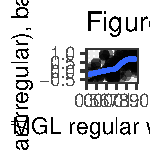
\includegraphics{figures/baseline_156-1.pdf}

The MGL weights correlate with the response odds, as seen in Figure 1.
Rácz, Beckner, Hay \& Pierrehumbert (2020) and Albright \& Hayes (2003)
likewise find that the minimal generalisations (rules) of the MGL are
more accurate in predicting participant responses than an instance-based
learner, despite the higher level of abstraction.

\hypertarget{the-esp-experiment}{%
\section{The ESP experiment}\label{the-esp-experiment}}

Rácz, Beckner, Hay \& Pierrehumbert (2020) ran a second online
experiment using the nonwords from the baseline experiment. Each
participant went through three blocks. First, in the pretest phase, they
responded to 52 standalone nonwords in a forced-choice task, similar to
the baseline experiment. Second, in the test phase, they responded to a
new set of 52 nonwords. This time they were playing against a co-player
and had to guess the coplayer's pick in each trial. Correct guesses were
rewarded with a point. Coplayer behaviour was based on the participant's
specific pretest behaviour and the baseline data. Third, in the posttest
phase, they responded to a new set of 52 nonwords, alone again.

Coplayers varied across two conditions. In terms of (A) rate of
regularisation, the coplayer had (i) the same regularisation rate as the
participant in the pretest, (ii) regularised 40\% more verbs, (iii)
regularised 40\% fewer verbs. Participants who regularised too much or
too little (so that the entire effect of this shift would have been
capped by the floor or the ceiling of the 52 verbs in the test) were
excluded. In terms of (B) lexical distribution, the coplayer regularised
the first n verbs (n depending on A) that were rated most regular in the
baseline task (the typical coplayer), the first n verbs that were rated
most irregular in the baseline task (the reversed coplayer), or n verbs
at random (the random coplayer).

\hypertarget{results-1}{%
\subsection{Results}\label{results-1}}

Rácz, Beckner, Hay \& Pierrehumbert (2020) found that the coplayer
changed participant behaviour. Nonword ratings shifted from the pretest
to the posttest. If participants rated words as highly regular in the
pretest, they rated these more irregular in the posttest, after
interacting with the reversed versus the typical coplayer. Since no
participant saw the same verb twice, this effect was due to lexical,
rather than word priming. The reversed coplayer used verbs in a certain
way, and the participant rated similar verbs in the posttest in a
certain way. The difference with the random coplayer was less clearcut.

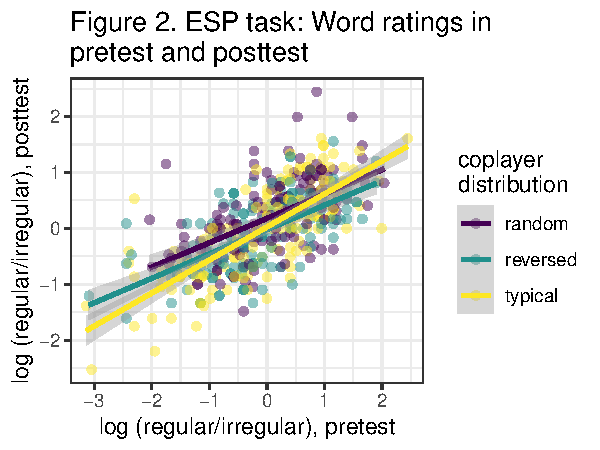
\includegraphics{figures/mainres1-1.pdf}

\hypertarget{what-goes-wrong-in-the-posttest}{%
\section{What goes wrong in the
posttest}\label{what-goes-wrong-in-the-posttest}}

Since the MGL weights highly correlate with participant responses that
lack coplayer influence, we see a similar distribution if we look at how
MGL prediction accuracy varies across coplayers in the posttest.

The main effect of interest is coplayer lexical distribution. The MGL
weight has a stronger effect on posttest responses if the participant
played a typical coplayer. This makes sense: a typical coplayer
reinforces existing lexical distributions. Why does the MGL get worse
after a reversed or random coplayer?

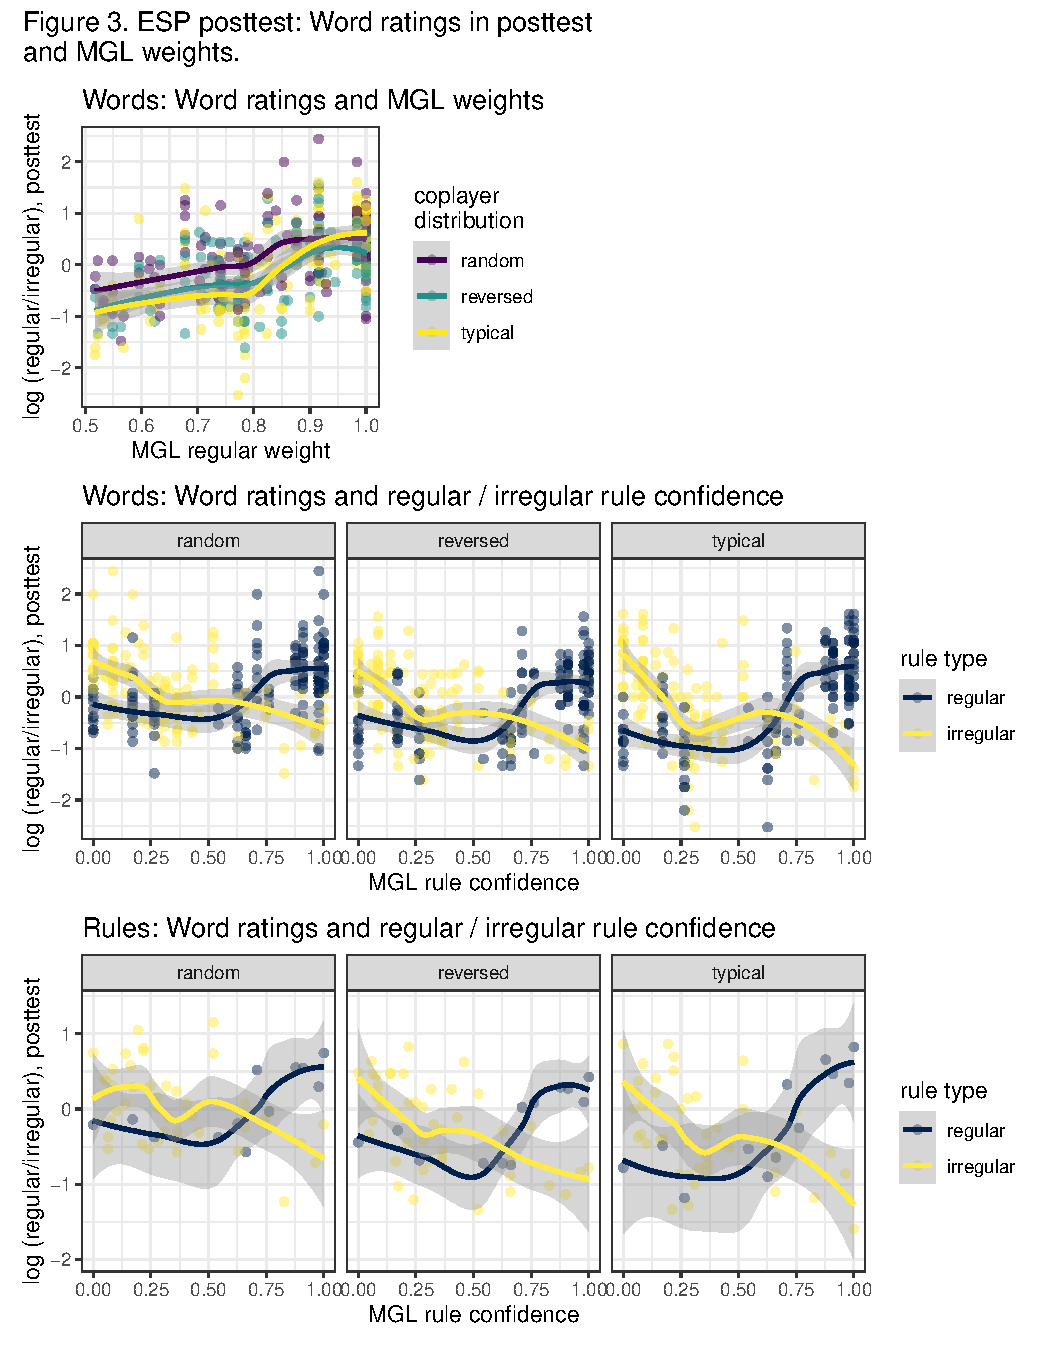
\includegraphics{figures/mglbreakdown1-1.pdf}

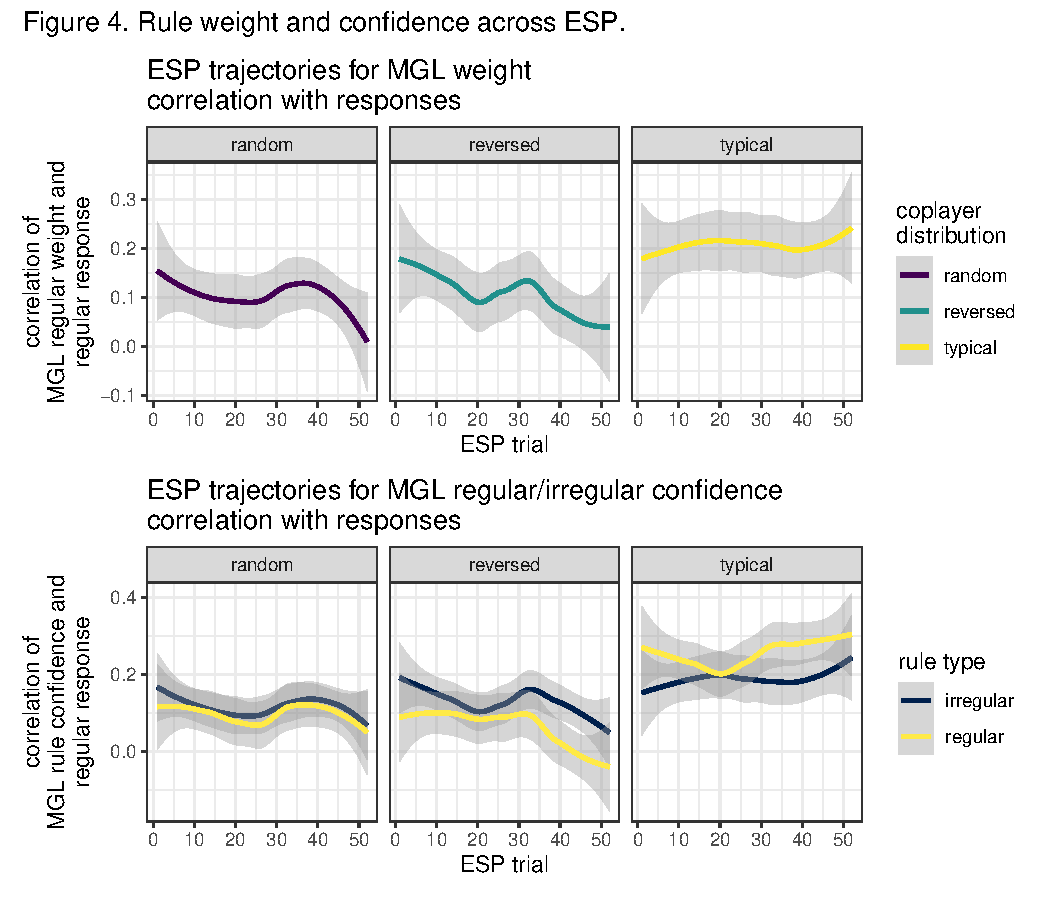
\includegraphics{figures/mglbreakdown2-1.pdf}

\hypertarget{modelling}{%
\section{Modelling}\label{modelling}}

Big rules overlap across esp and posttest.

\begin{table}
\centering
\caption{\label{tab:ruleoverlap}3. Rule overlaps for one participant}
\centering
\begin{tabular}[t]{lrl}
\toprule
rule & scope & phase\\
\midrule
\cellcolor{gray!10}{{}[] -> d  [D, J, N, S, T, Z, \_, b, d, f, g, h, k, l, m, n, p, s, t, v, z, \textasciitilde{}] \_} & \cellcolor{gray!10}{3510} & \cellcolor{gray!10}{esp, posttest}\\
{}[] -> d  [3, D, J, S, T, Z, \_, d, l, n, r, s, t, z] \_ & 3183 & esp, posttest\\
\cellcolor{gray!10}{{}[] -> d  [D, J, S, T, Z, \_, b, d, f, g, k, p, s, t, v, z, \textasciitilde{}] \_} & \cellcolor{gray!10}{2602} & \cellcolor{gray!10}{esp, posttest}\\
{}[] -> t  [D, J, S, T, Z, \_, d, s, t, z] \_ & 2020 & esp, posttest\\
\cellcolor{gray!10}{{}[] -> t  [J, S, T, f, k, p, s, t, \textasciitilde{}] \_} & \cellcolor{gray!10}{1779} & \cellcolor{gray!10}{esp, posttest}\\
\addlinespace
{}[] -> t  [d, n, t] \_ & 1545 & esp, posttest\\
\cellcolor{gray!10}{{}[] -> d  [3, D, S, T, Z, l, r, s, z] \_} & \cellcolor{gray!10}{1443} & \cellcolor{gray!10}{esp, posttest}\\
{}[] -> d  [J, S, T, s, t] \_ & 1364 & esp, posttest\\
\cellcolor{gray!10}{{}[] -> @d  t \_} & \cellcolor{gray!10}{959} & \cellcolor{gray!10}{esp, posttest}\\
{}[] -> d  [D, S, T, Z, n, s, z] \_ & 902 & esp, posttest\\
\addlinespace
\cellcolor{gray!10}{{}[] -> d  [D, S, T, Z, f, s, v, z] \_} & \cellcolor{gray!10}{712} & \cellcolor{gray!10}{esp, posttest}\\
{}[] -> d  [b, p] \_ & 214 & esp, posttest\\
\cellcolor{gray!10}{{}[] -> d  [b, m] \_} & \cellcolor{gray!10}{169} & \cellcolor{gray!10}{esp, posttest}\\
{}[] -> d  [3, @, a]n \_ & 135 & esp, posttest\\
\cellcolor{gray!10}{{}[] -> @d  [2, 3, 4, 6, @, A, E, Q, V, a, e, o, \{, »]d \_} & \cellcolor{gray!10}{99} & \cellcolor{gray!10}{esp, posttest}\\
\addlinespace
{}[] -> d  [2, 4, 6, e, i, o, u]m \_ & 63 & esp, posttest\\
\cellcolor{gray!10}{{}[] -> t  [E, I]l \_} & \cellcolor{gray!10}{46} & \cellcolor{gray!10}{esp, posttest}\\
I -> \{  [j, r, w]» \_ [N, m, n] & 45 & esp, posttest\\
\cellcolor{gray!10}{2 -> o  [D, J, S, T, Z, \_, d, l, n, r, s, t, z]» \_ [D, N, Z, m, n, v, z]} & \cellcolor{gray!10}{44} & \cellcolor{gray!10}{esp, posttest}\\
2 -> o  [D, Z, \_, d, l, n, r, z]» \_ [D, Z, \_, b, d, g, v, z] & 34 & esp, posttest\\
\addlinespace
\cellcolor{gray!10}{2 -> o  [N, j, l, m, n, r, w]» \_ [d, t]} & \cellcolor{gray!10}{22} & \cellcolor{gray!10}{esp, posttest}\\
2 -> o  [N, j, l, m, n, r, w]» \_ t & 14 & esp, posttest\\
\cellcolor{gray!10}{2 -> o  [S, Z, r]» \_ [d, n, t]} & \cellcolor{gray!10}{13} & \cellcolor{gray!10}{esp, posttest}\\
I -> \{  [D, S, T, Z, l, r, s, z]» \_ N & 10 & esp, posttest\\
\cellcolor{gray!10}{2 -> o  r» \_ [d, t]} & \cellcolor{gray!10}{9} & \cellcolor{gray!10}{esp, posttest}\\
\addlinespace
I -> \{  [b, m, v, w]» \_ [N, \_, b, d, g, m, n] & 8 & esp, posttest\\
\cellcolor{gray!10}{I -> \{  [N, g, j, w]» \_ [N, m, n]} & \cellcolor{gray!10}{5} & \cellcolor{gray!10}{esp, posttest}\\
2 -> o  [3, D, J, S, T, Z, \_, d, l, n, r, s, t, z]r» \_ [d, t] & 4 & esp, posttest\\
\cellcolor{gray!10}{i -> o  [D, J, N, S, T, Z, \_, b, d, f, g, h, j, k, l, m, n, p, r, s, t, v, w, z, \textasciitilde{}]» \_ [D, Z, l, v, z]} & \cellcolor{gray!10}{50} & \cellcolor{gray!10}{esp}\\
I -> \{  [D, J, S, T, Z, \_, d, l, n, r, s, t, z]» \_ N & 35 & esp\\
\addlinespace
\cellcolor{gray!10}{I -> \{  [D, S, T, Z, l, r, s, z]» \_ [J, N, \_, b, d, g, k, m, n, p, t, \textasciitilde{}]} & \cellcolor{gray!10}{15} & \cellcolor{gray!10}{esp}\\
I -> \{  [j, r, w]» \_ [N, m, n] & 15 & esp\\
\cellcolor{gray!10}{I -> \{  [D, J, S, T, Z, \_, d, l, n, r, s, t, z]» \_ Nk} & \cellcolor{gray!10}{12} & \cellcolor{gray!10}{esp}\\
ip -> Ept  [D, J, N, S, T, Z, \_, b, d, f, g, h, j, k, l, m, n, p, r, s, t, v, w, z, \textasciitilde{}]» \_ & 12 & esp\\
\cellcolor{gray!10}{2 -> o  [D, J, S, T, Z, \_, d, s, t, z]» \_ [D, N, Z, m, n, v, z]} & \cellcolor{gray!10}{9} & \cellcolor{gray!10}{esp}\\
\addlinespace
2 -> o  [D, Z, \_, d, l, n, r, z]» \_ v & 8 & esp\\
\cellcolor{gray!10}{{}[] -> t  [m, w]»El \_} & \cellcolor{gray!10}{7} & \cellcolor{gray!10}{esp}\\
il -> Elt  [D, J, N, S, T, Z, \_, b, d, f, g, k, m, n, p, s, t, v, z, \textasciitilde{}]» \_ & 7 & esp\\
\cellcolor{gray!10}{I -> \{  r» \_ N} & \cellcolor{gray!10}{6} & \cellcolor{gray!10}{esp}\\
I -> \{  [D, N, Z, \_, b, d, g, j, l, m, n, r, v, w, z]» \_ [N, m, n] & 83 & posttest\\
\addlinespace
\cellcolor{gray!10}{2 -> o  [D, N, S, T, Z, f, h, j, l, m, n, r, s, v, w, z]» \_ [d, n, t]} & \cellcolor{gray!10}{66} & \cellcolor{gray!10}{posttest}\\
I -> \{  [D, J, S, T, Z, \_, b, d, f, g, k, p, s, t, v, z, \textasciitilde{}]» \_ [N, m, n] & 58 & posttest\\
\cellcolor{gray!10}{2 -> o  [D, N, S, T, Z, f, m, n, s, v, z]» \_ [d, n, t]} & \cellcolor{gray!10}{36} & \cellcolor{gray!10}{posttest}\\
i -> o  [b, f, m, p, v, w]» \_ [D, J, S, T, Z, \_, b, d, f, g, k, p, s, t, v, z, \textasciitilde{}] & 30 & posttest\\
\cellcolor{gray!10}{I -> \{  [D, S, T, Z, f, h, j, l, r, s, v, w, z]» \_ [N, m, n]} & \cellcolor{gray!10}{22} & \cellcolor{gray!10}{posttest}\\
\addlinespace
2 -> o  [D, J, S, T, Z, \_, d, l, n, r, s, t, z]» \_ [D, N, Z, \_, b, d, g, m, n, v, z] & 18 & posttest\\
\cellcolor{gray!10}{{}[] -> @d  [D, J, S, T, Z, \_, b, d, f, g, k, p, s, t, v, z, \textasciitilde{}]»2d \_} & \cellcolor{gray!10}{13} & \cellcolor{gray!10}{posttest}\\
{}[] -> @d  [D, T, d, n, s, t, z]»2t \_ & 11 & posttest\\
\cellcolor{gray!10}{I -> \{  [D, J, S, T, Z, \_, b, d, f, g, k, p, s, t, v, z, \textasciitilde{}]r» \_ N} & \cellcolor{gray!10}{9} & \cellcolor{gray!10}{posttest}\\
ip -> Ept  [j, l, r, w]» \_ & 7 & posttest\\
\addlinespace
\cellcolor{gray!10}{{}[] -> t  [D, N, Z, \_, b, d, g, l, m, n, v, z]»3n \_} & \cellcolor{gray!10}{4} & \cellcolor{gray!10}{posttest}\\
ip -> Ept  [N, g, j, k, w]» \_ & 3 & posttest\\
\bottomrule
\end{tabular}
\end{table}

Does adjusting these rules help? We focus on reversed.

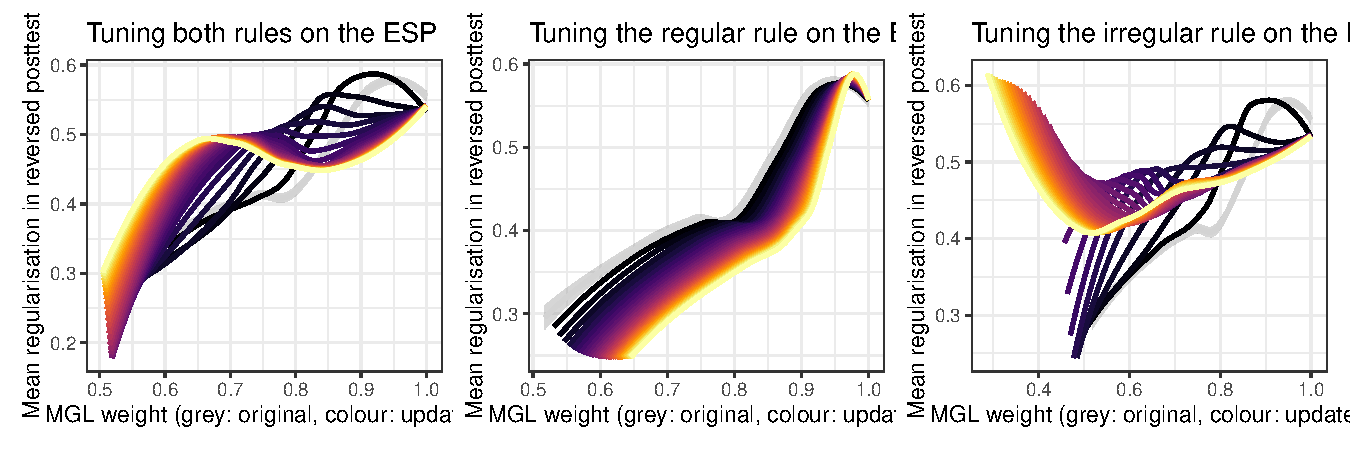
\includegraphics{figures/rulemove1-1.pdf}

\end{document}
